\section{Diffusion models}
\label{sec:diffusion-models}

Diffusion models are a way to sample from a target law \(p_0\) by starting from a reference law \(p_1\) that is easy to sample.
The abstract setup has two ingredients: a joint law for the endpoint pair \((X_0,X_1)\), with marginals \(p_0\) and \(p_1\), and a bridge that fills in the intermediate states.
We first set up that bridge abstractly and identify the reverse kernels needed for sampling.
We then specialize to Euclidean models, where the relevant reverse-time quantities can be learned by regression.
We then use the course sampling toolkit to build faster, guided, and diverse diffusion samplers within the same bridge notation.
The discrete-time ELBO appears as a grid-level rewriting of the same construction rather than as a separate starting point.

\subsection{Bridges and infinitesimal dynamics}
\label{subsec:diffusion-bridges-dynamics}

Let \(p_0\) be the law we want to sample and let \(p_1\) be a law from which sampling is easy.
The problem is to start from \(X_1\sim p_1\) and construct a reverse-time dynamics that ends at \(p_0\).
The abstract setup has two ingredients.
First choose a joint law for the endpoint pair \((X_0,X_1)\) with marginals \(p_0\) and \(p_1\).
Then choose a bridge that fills in the intermediate states.
This formulation works on a general state space, not just on \(\R^d\), so the Gaussian constructions used in continuous diffusion models are later specializations rather than the starting point.

For reverse-time sampling, the key object is the conditional bridge step from time \(t\) back to an earlier time \(s\).
In the one-sided form used throughout most of this chapter, the bridge provides the law of \(X_s\) given \((X_0,X_t)\).
The reverse kernel is obtained by averaging that bridge step against the posterior law of \(X_0\) given \(X_t\).
This bridge-first setup matches the general presentation in \citet[\S3.1]{holderrieth_erives_2026_intro_flow_matching} and \citet[\S5.3.2]{lai_song_kim_mitsufuji_ermon_2025_principles_diffusion}.

\subsubsection{Conditional and marginal probability paths}
\label{subsubsec:conditional-marginal-probability-paths}

Fix a state space \(\mathcal{X}\), for example \(\R^d\) in Euclidean models or a finite set in discrete models.
Let \(p_0\) and \(p_1\) be endpoint laws on \(\mathcal{X}\), with \(t=0\) corresponding to \(p_0\) and \(t=1\) corresponding to \(p_1\).
Choose a joint law \(\Gamma\) for \((X_0,X_1)\) with marginals \(p_0\) and \(p_1\); this is the coupling of the endpoints.
Then choose kernels \(K_{t\mid 0,1}(\cdot\mid x_0,x_1)\) describing the law of \(X_t\) given \((X_0,X_1)=(x_0,x_1)\).
Averaging those kernels against \(\Gamma\) gives the marginal path \(p_t\).

For reverse-time sampling, the key object is the conditional bridge step from \(t\) back to \(s\).
In the fully coupled formulation this is the law of \(X_s\) given \((X_0,X_1,X_t)\).
In many diffusion constructions it reduces to the law of \(X_s\) given \((X_0,X_t)\), which is the notation we use below.

\begin{definition}[Conditional and marginal probability paths]
\label{def:conditional-marginal-probability-path}
Let \((X_0,X_1)\sim \Gamma\), where \(\Gamma\) is a coupling of \((p_0,p_1)\).
A \emph{conditional probability path} is a family of Markov kernels \(\{K_{t\mid 0,1}(\,\cdot\,\mid x_0,x_1)\}_{t\in[0,1],\,(x_0,x_1)\in\mathcal{X}^2}\) such that
\[
  K_{0\mid 0,1}(\,\cdot\,\mid x_0,x_1)=\delta_{x_0},
  \qquad
  K_{1\mid 0,1}(\,\cdot\,\mid x_0,x_1)=\delta_{x_1},
\]
where \(\delta_{x}\) denotes the point mass at \(x\).
The \emph{marginal probability path} is the family of distributions
\begin{equation}
  p_t(A) \coloneqq \int_{\mathcal{X}^2} K_{t\mid 0,1}(A\mid x_0,x_1)\,\Gamma(dx_0,dx_1),
  \qquad A\subseteq\mathcal{X}\ \text{measurable}.
  \label{eq:marginal-path-general}
\end{equation}
\end{definition}

The same definition applies in continuous and discrete settings; on a finite state space the integrals are simply sums.
For reverse-time sampling, let \(K_{s\mid 0,1,t}\) denote the bridge step conditioned on \((X_0,X_1,X_t)\), and let
\[
  q_{0,1\mid t}(\cdot\mid x_t)\coloneqq \mathrm{Law}\bigl((X_0,X_1)\mid X_t=x_t\bigr).
\]
Then the reverse kernel from time \(t\) to time \(s\) is
\[
  K_{s\mid t}(A\mid x_t)
  =
  \int_{\mathcal{X}^2} K_{s\mid 0,1,t}(A\mid x_0,x_1,x_t)\,q_{0,1\mid t}(dx_0,dx_1\mid x_t).
\]
In many constructions, including the linear Gaussian path below, this reduces to conditioning only on \((X_0,X_t)\).
From that point on we write
\[
  q_{0\mid t}(\cdot\mid x_t)\coloneqq \mathrm{Law}(X_0\mid X_t=x_t),
\]
and \(K_{s\mid 0,t}\) for the corresponding bridge step conditioned on \((X_0,X_t)\).
The results below are written in this reduced notation; the fully coupled version is obtained by replacing \(X_0\) by \((X_0,X_1)\).
For \(0\le s\le t\le u\le 1\), the reverse kernels should also compose consistently in time.

\begin{definition}[Bridge-consistent reverse kernels]
\label{def:bridge-consistent-reverse-kernels}
Using the notation above, we say that the family \(\{K_{s\mid t}\}_{0\le s\le t\le 1}\) is \emph{bridge-consistent} if for every \(0\le s\le t\le u\le 1\) and every measurable set \(A\subseteq\mathcal{X}\),
\begin{equation}
  K_{s\mid t}(A\mid x_t)
  =
  \int_{\mathcal{X}} K_{s\mid 0,t}(A\mid x_0,x_t)\,q_{0\mid t}(dx_0\mid x_t).
  \label{eq:bridge-consistency-posterior}
\end{equation}
and
\begin{equation}
  K_{s\mid u}(A\mid x_u)
  =
  \int_{\mathcal{X}} K_{s\mid t}(A\mid x_t)\,K_{t\mid u}(dx_t\mid x_u),
  \label{eq:bridge-consistency-ck}
\end{equation}
\end{definition}

\Cref{eq:bridge-consistency-ck} says that reverse kernels compose correctly in time, just as forward Markov kernels do.
\Cref{eq:bridge-consistency-posterior} says how a single reverse step is built:
condition on the endpoint, take the corresponding bridge step, and then average over the posterior of that endpoint given the current state.
In discrete models the same formulas hold with sums in place of integrals, and the resulting reverse dynamics is usually implemented by time-inhomogeneous jump kernels.
In Euclidean models it is more convenient to pass next to infinitesimal notation.

\subsubsection{Exact distributional posterior learning}

Before making any tractability reduction, it is worth spelling out the exact idealization.
We state it in the reduced notation just introduced; the fully coupled endpoint version is identical.
Suppose that at each time \(t\) we could learn the full conditional law
\[
  q_{0\mid t}(\cdot\mid x_t)=\mathrm{Law}(X_0\mid X_t=x_t)
\]
of the endpoint given the current state.
Then reverse-time sampling would proceed in two steps:
first sample an endpoint from that conditional law, then take a bridge step conditioned on the sampled endpoint.
This is a genuinely distributional model, because the learned object is the whole posterior law rather than a smaller statistic derived from it.

\begin{proposition}[Exact reverse kernels transport the forward path]
\label{prop:reverse-kernels-transport-general}
For every \(0\le s\le t\le 1\) and every measurable set \(A\subseteq\mathcal{X}\),
\[
  p_s(A)
  =
  \int_{\mathcal{X}} K_{s\mid t}(A\mid x_t)\,p_t(dx_t).
\]
\end{proposition}
\begin{proof}
By the law of total probability,
\[
  \int_{\mathcal{X}} K_{s\mid t}(A\mid x_t)\,p_t(dx_t)
  =
  \mathbb{P}(X_s\in A)
  =
  p_s(A).
\]
\end{proof}

\begin{theorem}[Distributional posterior learning is exact on any grid]
\label{thm:distributional-posterior-learning}
Fix any decreasing time grid \(1=t_K>\cdots>t_0=0\).
Suppose a model returns the exact conditional law
\[
  q_{0\mid t_k}(\cdot\mid x)=\mathrm{Law}(X_0\mid X_{t_k}=x)
\]
at every grid time.
Initialize \(\hat X_{t_K}\sim p_1\), and for \(k=K,\dots,1\) generate the reverse chain by
\[
  \tilde X_0^{(k)} \mid \hat X_{t_k}=x
  \sim
  q_{0\mid t_k}(\cdot\mid x),
  \qquad
  \hat X_{t_{k-1}} \mid \bigl(\tilde X_0^{(k)}=x_0,\hat X_{t_k}=x\bigr)
  \sim
  K_{t_{k-1}\mid 0,t_k}(\cdot\mid x_0,x).
\]
Then \(\hat X_{t_k}\sim p_{t_k}\) for every \(k\).
In particular \(\hat X_{t_0}\sim p_0\).
\end{theorem}
\begin{proof}
Conditionally on \(\hat X_{t_k}=x\), we first sample \(\tilde X_0^{(k)}\sim q_{0\mid t_k}(\cdot\mid x)\) and then sample \(\hat X_{t_{k-1}}\) from the bridge conditioned on that endpoint.
Therefore, for any measurable \(A\subseteq\mathcal{X}\),
\[
  \mathbb{P}\bigl(\hat X_{t_{k-1}}\in A\mid \hat X_{t_k}=x\bigr)
  =
  \int_{\mathcal{X}} K_{t_{k-1}\mid 0,t_k}(A\mid x_0,x)\,q_{0\mid t_k}(dx_0\mid x)
  =
  K_{t_{k-1}\mid t_k}(A\mid x),
\]
where the second equality is the posterior-averaging identity \eqref{eq:bridge-consistency-posterior}.
Assume inductively that \(\hat X_{t_k}\sim p_{t_k}\).
Then by \Cref{prop:reverse-kernels-transport-general},
\[
  \mathbb{P}(\hat X_{t_{k-1}}\in A)
  =
  \int_{\mathcal{X}} K_{t_{k-1}\mid t_k}(A\mid x)\,p_{t_k}(dx)
  =
  p_{t_{k-1}}(A).
\]
Starting from \(\hat X_{t_K}\sim p_1\), induction gives the claim for every grid point.%
\end{proof}

This theorem is domain-agnostic.
It applies just as well on \(\R^d\) as on a finite state space.
The practical question is therefore not whether full posterior learning would be correct, but which part of that exact distributional picture can be represented tractably.
On a finite state space, the learned object can sometimes literally be a simplex vector.
On \(\R^d\), the full posterior is genuinely infinite-dimensional, so the tractability move is to replace it by posterior moments that still determine the marginal dynamics.
From this point on, the Euclidean development makes that reduction explicit.

\subsubsection{Stochastic interpolants and Gaussian bridges}

When \(\mathcal{X}=\R^d\), one flexible way to design conditional paths is the \emph{stochastic interpolant} framework of \citet[Def.~1]{albergo_boffi_vanden_eijnden_2025_stochastic_interpolants}.
The construction answers three questions:
how to couple the endpoint laws, how to interpolate between sampled endpoints, and how much additional bridge noise to add along the way.
It specifies a random variable \(X_t\) of the form
\begin{equation}
  X_t \coloneqq I(t,X_0,X_1) + \gamma(t)\xi,
  \label{eq:stochastic-interpolant-bridge}
\end{equation}
where \((X_0,X_1)\) is a coupling of \((p_0,p_1)\), \(\xi\sim\mathcal{N}(0,I_d)\) is independent noise, \(I(0,x_0,x_1)=x_0\), \(I(1,x_0,x_1)=x_1\), and \(\gamma(0)=\gamma(1)=0\).
The structural results below depend only on this path specification.
The main continuous-diffusion specialization is the linear Gaussian family, because in that case the posterior summaries and reverse-time dynamics become completely explicit.
For the Gaussian conditional-path specialization used in flow matching, see also \citet[\S\S3.1 and 4]{lipman_chen_ben_hamu_nickel_le_2023_flow_matching}.
In that specialization,
\begin{equation}
  X_t = \alpha(t)X_0 + \sigma(t) Z,
  \qquad
  Z\sim\mathcal{N}(0,I_d)\ \text{independent of }X_0.
  \label{eq:gaussian-bridge-path}
\end{equation}
Here \(\alpha(0)=1\), \(\alpha(1)=0\), \(\sigma(0)=0\), and \(\sigma(1)=1\).
This still sits inside the stochastic-interpolant framework.
In particular, if we take the linear interpolant \(I(t,x_0,x_1)=(1-t)x_0+tx_1\), let \(X_1\sim\mathcal{N}(0,I_d)\), and keep a nonzero bridge noise \(\gamma(t)\xi\), then conditioned on \(X_0\) the resulting path is Gaussian with
\[
  \alpha(t)=1-t,
  \qquad
  \sigma(t)^2=t^2+\gamma(t)^2.
\]
We therefore parametrize the running example directly by \(\alpha\) and \(\sigma\), since those are the quantities that enter the conditional laws and reverse-time formulas.

Conditioned on \(X_0=x_0\), the law of \(X_t\) is Gaussian:
\begin{equation}
  X_t \mid X_0=x_0 \sim \mathcal{N}\bigl(\alpha(t)x_0,\ \sigma(t)^2 I_d\bigr).
  \label{eq:gaussian-conditional-path}
\end{equation}
The endpoint conditions imply
\[
  X_1 \mid X_0=x_0 \sim \mathcal{N}(0,I_d)=p_1,
  \qquad
  X_0 \mid X_0=x_0 = x_0,
\]
so the conditional path really does end at the full reference law \(p_1\), independently of \(x_0\).
\eqref{eq:gaussian-conditional-path} can be read as the density of the conditional kernel \(K_{t\mid 0}(\,\cdot\,\mid x_0)\), which couples the endpoint \(x_0\) to the reference law through a linear Gaussian bridge.
The corresponding marginal density is the mixture
\begin{equation}
  p_t(x)
  =
  \int_{\R^d} K_{t\mid 0}(x\mid x_0)\,p_0(x_0)\,dx_0.
  \label{eq:marginal-mixture-path}
\end{equation}
The conditional/marginal distinction in \eqref{eq:gaussian-conditional-path}--\eqref{eq:marginal-mixture-path} is also the starting point for flow matching \citep[\S3.1]{lipman_chen_ben_hamu_nickel_le_2023_flow_matching}.
\Cref{fig:diffusion-cond-vs-marg} illustrates the induced conditional and marginal laws.

\begin{figure}[t]
  \centering
  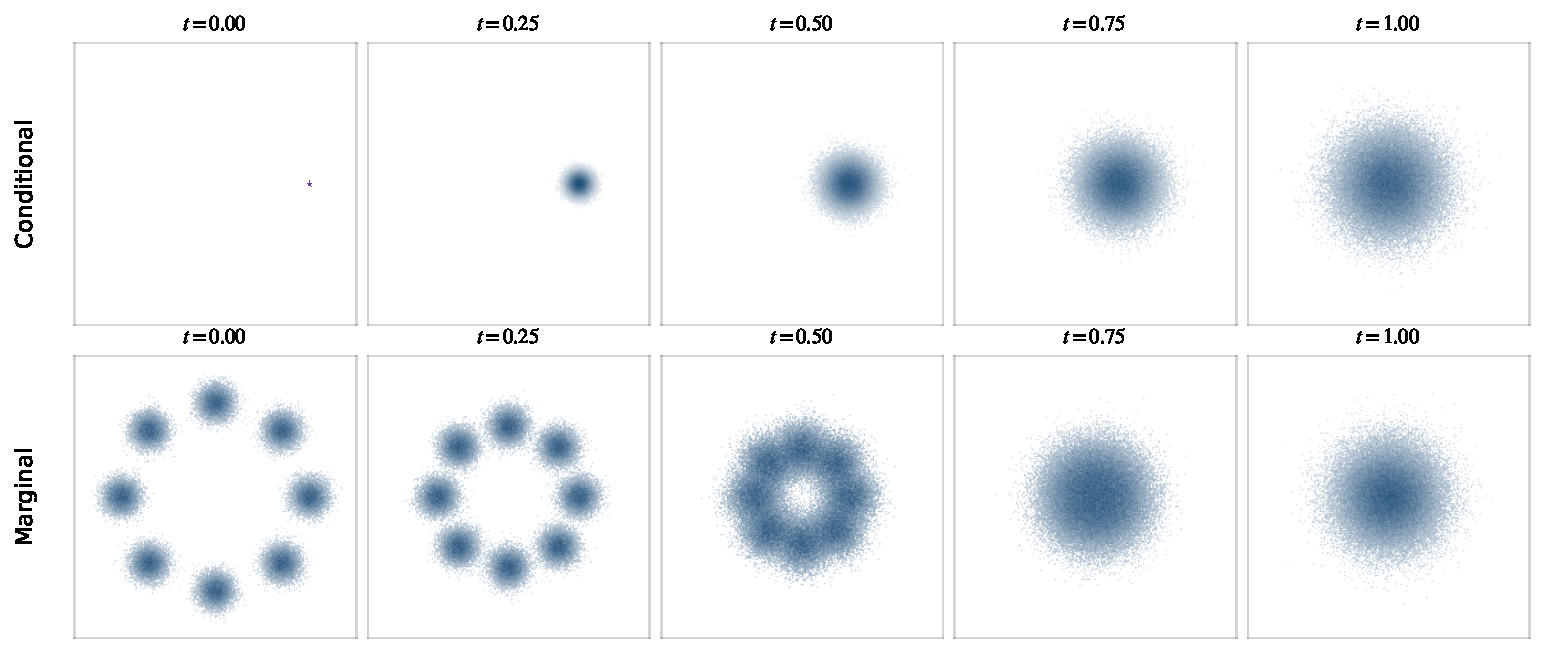
\includegraphics[width=\textwidth]{figures/main_notes/diffusion_models/fig_diffusion_conditional_vs_marginal.pdf}
  \caption{The Gaussian conditional path \eqref{eq:gaussian-conditional-path} for a fixed \(x_0\) (top row) and the induced marginal law \(p_t\) when \(X_0\sim p_0\) (bottom row), illustrated here for the simple choice \(\alpha(t)=1-t\) and \(\sigma(t)=t\).
  Sampling starts from \(p_1\) at \(t=1\) and runs the reverse-time dynamics back to \(t=0\).}
  \label{fig:diffusion-cond-vs-marg}
\end{figure}

The probability path induces a posterior distribution at every time: conditioning on \(X_t=x\) produces a conditional law for the retained endpoint variables, and, if we use a construction like \eqref{eq:stochastic-interpolant-bridge}, for the auxiliary latent variables as well.
This posterior is the exact object from which the reverse kernel is obtained, by the averaging identity above.
In the Euclidean setting we typically do not try to model the full posterior on all latent variables directly.
Instead, the deterministic and stochastic dynamics below depend only on conditional expectations under this posterior, and those expectations are exactly the infinitesimal quantities needed to generate the marginal path.

\subsubsection{Velocity, Endpoint Means, and Score Recovery}

For reverse-time simulation we need a field that depends only on the current state \(x\), not on the hidden variables used to generate the bridge.
The Euclidean tractability move is therefore to replace the full posterior law \(q_{0\mid t}(\cdot\mid x)\) by conditional expectations under it.
For a differentiable interpolant, define the time derivative
\[
  \dot X_t \coloneqq \partial_t I(t,X_0,X_1) + \gamma'(t)\xi,
\]
which still depends on the latent variables and so cannot be used directly as a state-dependent drift.
Its posterior mean is the \emph{velocity field}
\begin{equation}
  b(t,x) \coloneqq \E[\dot X_t \mid X_t=x].
  \label{eq:si-velocity-def}
\end{equation}
This is the primary posterior summary in the continuous-time theory.
See \citet[\S4.1, eqs.~(38)--(40)]{holderrieth_erives_2026_intro_flow_matching} for the same velocity/score/endpoint-mean conversion pattern in a general bridge exposition.
For the linear Gaussian bridge \eqref{eq:gaussian-bridge-path}, it is also useful to introduce the posterior mean of the endpoint at time \(0\),
\begin{equation}
  m(t,x) \coloneqq \E[X_0\mid X_t=x].
  \label{eq:si-endpoint-mean-x0-def}
\end{equation}
Once these two summaries are in hand, the score will follow algebraically from the same Gaussian identities.
For the linear Gaussian bridge \eqref{eq:gaussian-bridge-path}, we have
\[
  \dot X_t = \alpha'(t)X_0 + \sigma'(t)Z,
\]
so \(b(t,x)=\E[\alpha'(t)X_0+\sigma'(t)Z\mid X_t=x]\).
Moreover, conditioning on \((X_0,X_t)=(x_0,x)\) yields
\[
  \E[\dot X_t\mid X_0=x_0,X_t=x]
  =
  \alpha'(t)x_0
  +
  \frac{\sigma'(t)}{\sigma(t)}\bigl(x-\alpha(t)x_0\bigr),
\]
which is the closed-form conditional vector field used in conditional flow matching.
The score field \(s(t,x)\coloneqq \nabla\log p_t(x)\) is then determined by \(b\) as well.

\begin{proposition}[Derived endpoint mean and score for the linear Gaussian bridge]
\label{prop:score-from-endpoint-mean}
Assume \eqref{eq:gaussian-bridge-path} holds with smooth functions \(\alpha,\sigma\) such that \(\sigma(t)>0\) and
\[
  D(t)\coloneqq \alpha(t)\sigma'(t)-\sigma(t)\alpha'(t)\neq 0
\]
for \(t\in(0,1]\).
Fix \(t\in(0,1]\).
Assume \(x\mapsto K_{t\mid 0}(x\mid x_0)\) is \(C^1\) for every \(x_0\), that differentiation with respect to \(x\) may be passed through the mixture formula \eqref{eq:marginal-mixture-path}, and that \(p_t(x)>0\) at the points where the score identity is evaluated.
Then:
\begin{enumerate}[leftmargin=*]
  \item The endpoint posterior mean is determined by the velocity:
  \begin{equation}
    m(t,x) = \frac{\sigma'(t)x-\sigma(t)b(t,x)}{D(t)}.
    \label{eq:endpoint-mean-from-velocity}
  \end{equation}
  \item The score can be written in terms of the endpoint mean (equivalently, in terms of \(b\)):
  \begin{equation}
    \nabla\log p_t(x)
    =
    -\frac{1}{\sigma(t)^2}\Bigl(x-\alpha(t)\,m(t,x)\Bigr)
    =
    \frac{\alpha'(t)x-\alpha(t)b(t,x)}{\sigma(t)D(t)}.
    \label{eq:score-from-endpoint-mean}
  \end{equation}
\end{enumerate}
\end{proposition}
\begin{proof}
Define
\[
  n(t,x)\coloneqq \E[Z\mid X_t=x].
\]
Taking conditional expectations in \eqref{eq:gaussian-bridge-path} gives
\[
  x = \alpha(t)\E[X_0\mid X_t=x] + \sigma(t)\E[Z\mid X_t=x]
  = \alpha(t)m(t,x)+\sigma(t)n(t,x).
\]
Likewise,
\[
  b(t,x)=\alpha'(t)m(t,x)+\sigma'(t)n(t,x).
\]
Eliminating \(n(t,x)\) from these two equations yields
\[
  D(t)m(t,x)=\sigma'(t)x-\sigma(t)b(t,x),
\]
which proves \eqref{eq:endpoint-mean-from-velocity}.

For the score, conditioned on \(X_0\), \eqref{eq:gaussian-conditional-path} gives the density
\[
  K_{t\mid 0}(x\mid X_0)
  \propto
  \exp\!\left(-\frac{1}{2\sigma(t)^2}\norm{x-\alpha(t)X_0}_2^2\right).
\]
Differentiating with respect to \(x\) yields
\[
  \nabla_x\log K_{t\mid 0}(x\mid X_0)
  =
  -\frac{x-\alpha(t)X_0}{\sigma(t)^2}.
\]
By \eqref{eq:marginal-mixture-path} and differentiation under the integral sign,
\[
  \nabla p_t(x)
  =
  \int_{\R^d}\nabla_x K_{t\mid 0}(x\mid x_0)\,p_0(x_0)\,dx_0.
\]
Since \(p_t(x)>0\), we may divide by \(p_t(x)\) and use \(\nabla_x K_{t\mid 0}=K_{t\mid 0}\nabla_x\log K_{t\mid 0}\) to obtain
\begin{align*}
  \nabla\log p_t(x)
  &=
  \frac{1}{p_t(x)}
  \int_{\R^d}\nabla_x K_{t\mid 0}(x\mid x_0)\,p_0(x_0)\,dx_0 \\
  &=
  \int_{\R^d}\nabla_x\log K_{t\mid 0}(x\mid x_0)\,
  \frac{K_{t\mid 0}(x\mid x_0)\,p_0(x_0)}{p_t(x)}\,dx_0.
\end{align*}
The factor multiplying \(\nabla_x\log K_{t\mid 0}\) is exactly the posterior density of \(X_0\) given \(X_t=x\), so this is the Fisher-type identity
\[
  \nabla\log p_t(x)
  =
  \E\!\left[\nabla_x\log K_{t\mid 0}(x\mid X_0)\mid X_t=x\right].
\]
Substituting the Gaussian score from above gives
\[
  \nabla\log p_t(x)
  =
  -\frac{1}{\sigma(t)^2}\,\E\!\left[x-\alpha(t)X_0\mid X_t=x\right]
  =
  -\frac{1}{\sigma(t)^2}\Bigl(x-\alpha(t)m(t,x)\Bigr),
\]
which is the first identity in \eqref{eq:score-from-endpoint-mean}.
Using \(x-\alpha(t)m(t,x)=\sigma(t)n(t,x)\) and eliminating \(m(t,x)\) instead gives
\[
  D(t)n(t,x)=\alpha(t)b(t,x)-\alpha'(t)x,
\]
hence
\[
  \nabla\log p_t(x)
  =
  -\frac{n(t,x)}{\sigma(t)}
  =
  \frac{\alpha'(t)x-\alpha(t)b(t,x)}{\sigma(t)D(t)}.
\]
This is the second identity in \eqref{eq:score-from-endpoint-mean}.
\end{proof}

The practical lesson is that the Gaussian bridge turns the full posterior law into a small menu of interchangeable posterior summaries.
One may learn the velocity field, the endpoint posterior mean, the Gaussian innovation predictor, or the score.
For this bridge these are not different conceptual objects; they are linear reparameterizations of the same posterior information.

\subsubsection{Density evolution and common-marginal dynamics}
\label{subsubsec:diffusion-density-evolution}

The velocity field \(b\) transports the marginal density \(p_t\).
One realization of this path is the deterministic probability-flow ODE with drift \(b\), and in flow matching this is the core marginalization trick: one can define a marginal vector field by averaging simple conditional velocities under the posterior, and this marginal vector field exactly generates the marginal probability path \citep[\S3.1]{lipman_chen_ben_hamu_nickel_le_2023_flow_matching}; see also \citet[Thm.~11]{holderrieth_erives_2026_intro_flow_matching}.

\begin{proposition}[Transport equation for the bridge marginals]
\label{prop:si-transport-equation}
Assume \(t\mapsto X_t\) is differentiable almost surely and that \(X_t\) has a density \(p_t\) for every \(t\in[0,1]\).
Let \(b\) be defined by \eqref{eq:si-velocity-def}.
Then \(p_t\) satisfies
\begin{equation}
  \partial_t p_t(x) + \nabla\cdot\bigl(b(t,x)p_t(x)\bigr)=0.
  \label{eq:si-transport-equation}
\end{equation}
\end{proposition}
\begin{proof}
Let \(\varphi\in C_0^\infty(\R^d)\).
Differentiate \(\varphi(X_t)\) using \(\dot X_t\) and take expectations:
\[
  \frac{d}{dt}\E[\varphi(X_t)]
  =
  \E\!\left[\ip{\nabla\varphi(X_t)}{\dot X_t}\right]
  =
  \E\!\left[\ip{\nabla\varphi(X_t)}{\E[\dot X_t\mid X_t]}\right]
  =
  \int_{\R^d}\ip{\nabla\varphi(x)}{b(t,x)}p_t(x)\,dx.
\]
Integrating by parts yields the weak form of \eqref{eq:si-transport-equation}.
\end{proof}

Once \(p_t\) and \(b\) are fixed, there is no reason to privilege a single trajectory-level dynamics.
The same forward law can be realized by a whole family of reverse-time diffusions and ODEs.
For sampling, the stochastic realizations are especially natural, while the probability-flow ODE appears as the zero-noise member of the same family.
This common-marginal viewpoint is formalized by \citet[\S2]{albergo_boffi_vanden_eijnden_2025_stochastic_interpolants} and \citet[Thm.~17]{holderrieth_erives_2026_intro_flow_matching}.

\begin{proposition}[A common-marginal family of dynamics]
\label{prop:si-family-of-sdes}
Assume that for each \(t\in(0,1)\), the density \(p_t\) is \(C^2\) and strictly positive on \(\R^d\).
Let \(s(t,x)\coloneqq\nabla\log p_t(x)\), and assume the Fokker--Planck equations below are well posed for the initial data considered.
Fix any continuous schedule \(\varepsilon:[0,1]\to[0,\infty)\) and define
\begin{equation}
  b_{\mathrm{fwd}}(t,x) \coloneqq b(t,x) + \varepsilon(t)s(t,x),
  \qquad
  b_{\mathrm{rev}}(t,x) \coloneqq b(t,x) - \varepsilon(t)s(t,x).
  \label{eq:si-forward-backward-drifts}
\end{equation}
Consider the forward and reverse-time dynamics
\begin{equation}
  dY_t^{\mathrm{fwd}}=b_{\mathrm{fwd}}(t,Y_t^{\mathrm{fwd}})\,dt+\sqrt{2\,\varepsilon(t)}\,dB_t,
  \qquad
  dY_t^{\mathrm{rev}}=b_{\mathrm{rev}}(t,Y_t^{\mathrm{rev}})\,dt+\sqrt{2\,\varepsilon(t)}\,dB_t,
  \label{eq:si-forward-backward-sdes}
\end{equation}
where the second equation is simulated backward in time from \(t=1\) to \(t=0\).
When \(\varepsilon\equiv 0\), these reduce to deterministic ODEs with drift \(b\).
Then:
\begin{enumerate}[leftmargin=*]
  \item If \(Y_0^{\mathrm{fwd}}\sim p_0\), then the time-marginal density of \((Y_t^{\mathrm{fwd}})\) is \(p_t\) for every \(t\in[0,1]\).
  \item If \(Y_1^{\mathrm{rev}}\sim p_1\), then the reverse-time marginal density of \((Y_t^{\mathrm{rev}})\) at time \(t\) is also \(p_t\).
\end{enumerate}
\end{proposition}
\begin{proof}
If \(\varepsilon\equiv 0\), then the first claim is exactly the transport equation \eqref{eq:si-transport-equation} written in trajectory form.
Assume now that \(\varepsilon\) is arbitrary.
The density \(\rho\) of \((Y_t^{\mathrm{fwd}})\) then satisfies the forward Fokker--Planck equation
\[
  \partial_t \rho + \nabla\cdot\bigl((b+\varepsilon s)\rho\bigr) = \varepsilon \Delta\rho.
\]
To identify the solution, observe that \(p_t\) itself satisfies the same PDE:
\[
  \partial_t p_t + \nabla\cdot\bigl((b+\varepsilon s)p_t\bigr)
  =
  \partial_t p_t + \nabla\cdot(bp_t) + \varepsilon\nabla\cdot(sp_t).
\]
By \eqref{eq:si-transport-equation}, the first two terms sum to zero, while
\[
  \nabla\cdot(sp_t)
  =
  \nabla\cdot\bigl((\nabla\log p_t)p_t\bigr)
  =
  \nabla\cdot(\nabla p_t)
  =
  \Delta p_t.
\]
Hence \(p_t\) solves the forward Fokker--Planck equation with initial condition \(p_0\).
By well posedness, \(\rho_t=p_t\) for all \(t\in[0,1]\).

For the second claim, set \(\tau\coloneqq 1-t\) and define \(\bar p_\tau(x)\coloneqq p_{1-\tau}(x)\).
Then
\[
  \partial_\tau \bar p_\tau(x)
  =
  -\partial_t p_t(x)\vert_{t=1-\tau}
  =
  \nabla\cdot\bigl(b(1-\tau,x)\bar p_\tau(x)\bigr)
\]
by \eqref{eq:si-transport-equation}.
Now consider the forward-in-\(\tau\) process associated with backward simulation in \(t\):
\[
  d\bar Y_\tau
  =
  -b_{\mathrm{rev}}(1-\tau,\bar Y_\tau)\,d\tau
  +
  \sqrt{2\,\varepsilon(1-\tau)}\,d\bar B_\tau.
\]
Its density \(\bar \rho_\tau\) satisfies
\[
  \partial_\tau \bar \rho_\tau
  +
  \nabla\cdot\bigl(-b_{\mathrm{rev}}(1-\tau,\cdot)\bar \rho_\tau\bigr)
  =
  \varepsilon(1-\tau)\Delta\bar \rho_\tau.
\]
Using \(b_{\mathrm{rev}}=b-\varepsilon s\), the candidate path \(\bar p_\tau\) obeys
\[
  \partial_\tau \bar p_\tau
  +
  \nabla\cdot\bigl((-b+\varepsilon s)(1-\tau,\cdot)\bar p_\tau\bigr)
  =
  \varepsilon(1-\tau)\nabla\cdot\bigl(s(1-\tau,\cdot)\bar p_\tau\bigr)
  =
  \varepsilon(1-\tau)\Delta\bar p_\tau.
\]
Thus \(\bar p_\tau\) solves the forward Fokker--Planck equation for the time-reversed simulation, with initial condition \(\bar p_0=p_1\).
By well posedness, \(\bar \rho_\tau=\bar p_\tau\).
Translating back to the original time variable \(t\) yields the stated reverse-time simulation property.
\end{proof}

\begin{corollary}[Langevin as a stationary-path special case]
\label{cor:langevin-stationary-path}
Suppose \(p_t\equiv \pi\) is constant in time, \(b\equiv 0\), and \(\varepsilon(t)\equiv 1\).
Then the forward member of \eqref{eq:si-forward-backward-sdes} is
\[
  dY_t = \nabla\log \pi(Y_t)\,dt + \sqrt{2}\,dB_t,
\]
which is exactly the overdamped Langevin diffusion from \Cref{subsubsec:langevin-diffusion}, and every marginal law is \(\pi\).
\end{corollary}
This is the course-level payoff of the common-marginal viewpoint.
The same drift-noise template governs stationary MCMC and time-inhomogeneous diffusion samplers; what changes is whether the target law is fixed or moves along the bridge.

\begin{figure}[t]
  \centering
  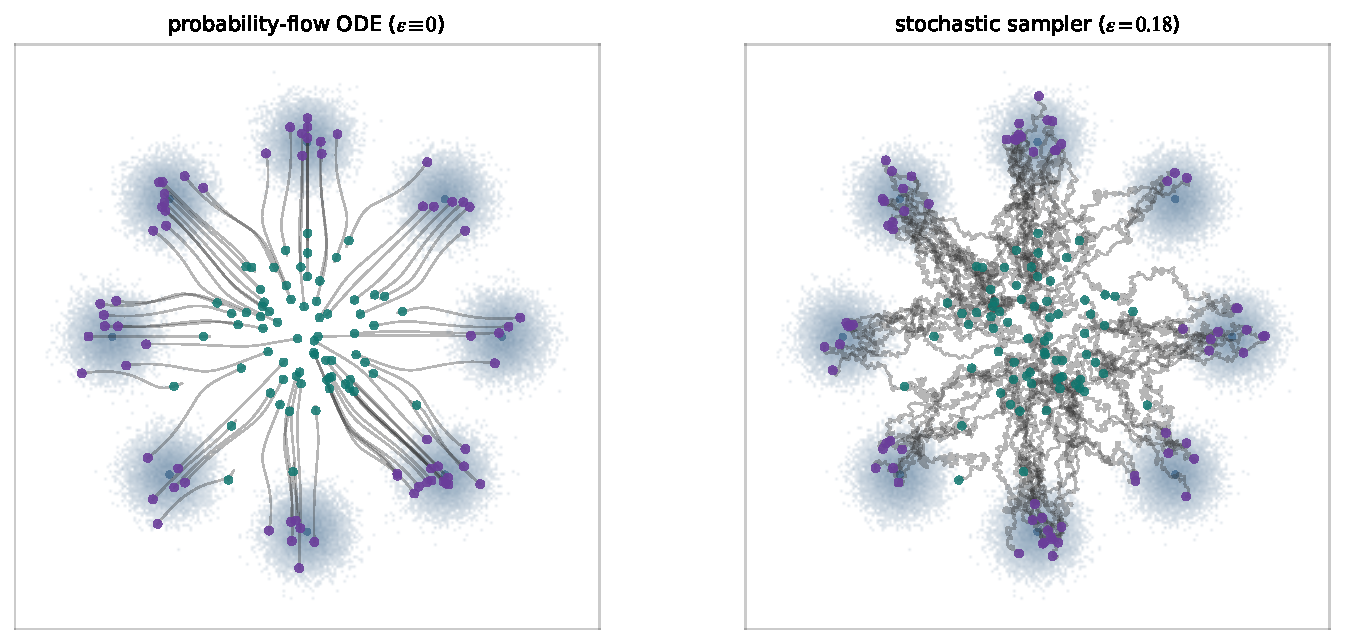
\includegraphics[width=\textwidth]{figures/main_notes/diffusion_models/fig_diffusion_reverse_dynamics.pdf}
  \caption{Reverse-time simulation from \(p_1\) back to \(p_0\) for a toy two-dimensional data distribution.
  Different choices of the noise schedule \(\varepsilon\) in \eqref{eq:si-forward-backward-sdes} produce different sample trajectories while preserving the same marginal path \(p_t\).
  The probability-flow ODE is the zero-noise case \(\varepsilon\equiv 0\).}
  \label{fig:diffusion-reverse-dynamics}
\end{figure}

\subsection{Regression and reverse-time simulation}
\label{subsec:diffusion-regression-simulation}

Once the exact bridge picture has been reduced to tractable posterior summaries, the practical problem is to learn those summaries and discretize the resulting reverse-time dynamics.
In Euclidean models this means regressing infinitesimal objects such as the velocity field and, when the bridge does not provide an explicit conversion formula, either the score itself or another summary from which the score can be recovered.
After time discretization the same bridge can also be written as a latent-path model with an ELBO objective, but that is a later reformulation of the same bridge rather than the starting point.

\subsubsection{Reverse-time sampling as regression}

The reverse-time family in \Cref{prop:si-family-of-sdes} involves both the velocity field \(b(t,x)\) and the score \(s(t,x)=\nabla\log p_t(x)\).
In principle one could instead parameterize the full posterior law \(q_{0\mid t}(\cdot\mid x)\) and use the exact distributional sampler from \Cref{thm:distributional-posterior-learning}.
Euclidean models usually do not do that, because the learned object would be a full conditional distribution on \(\R^d\) at every time.
This is the Euclidean tractability move from the posterior viewpoint.
Rather than parameterizing the full posterior, we ask for lower-dimensional summaries of it.
One natural summary is the conditional expectation \(b(t,x)=\E[\dot X_t\mid X_t=x]\), which is exactly the marginal velocity appearing in the transport equation and in flow matching.
For the linear Gaussian bridge, \Cref{prop:score-from-endpoint-mean} shows that both the score and the posterior mean of the \(t=0\) endpoint are explicit functions of that same velocity field.
That special algebraic reduction is the running example in this subsection.
Outside such specializations, learning \(b\) alone does not in general determine the reverse-time SDE: one also needs either a separate score model or another bridge-specific relation that recovers the score from the learned summary.
Once that reduction has been made, two practical questions remain:
how to learn the summary, and how to discretize the reverse-time dynamics determined by it.

For a general stochastic interpolant, the regression target is the conditional velocity $\dot X_t$ from \eqref{eq:si-velocity-def}.
From this point onward we use the linear Gaussian bridge as the running example, because it makes the recovery formulas completely explicit:
\[
  m(t,x)=\frac{\sigma'(t)x-\sigma(t)b(t,x)}{D(t)},
  \qquad
  \nabla\log p_t(x)=\frac{\alpha'(t)x-\alpha(t)b(t,x)}{\sigma(t)D(t)},
  \qquad
  D(t)=\alpha(t)\sigma'(t)-\sigma(t)\alpha'(t).
\]
At the level of updates, three parts of the course now line up:
\[
  \text{gradient descent:}\qquad x_{k+1}=x_k-\eta \nabla f(x_k),
\]
\[
  \text{ULA:}\qquad x_{k+1}=x_k+\eta \nabla\log \pi(x_k)+\sqrt{2\eta}\,\xi_k,
  \qquad \xi_k\sim\mathcal{N}(0,I_d),
\]
\[
  \text{reverse diffusion:}\qquad
  x_{t_k}
  =
  x_{t_{k+1}}
  +
  \Delta t\,\bigl(b(t,x_{t_{k+1}})-\varepsilon(t)s(t,x_{t_{k+1}})\bigr)
  +
  \sqrt{2\,\varepsilon(t)|\Delta t|}\,\xi_k,
\]
with $\Delta t=t_k-t_{k+1}<0$.
The optimization update uses only drift, Langevin adds calibrated noise to target a fixed distribution, and diffusion samplers use the same drift-noise template for a time-varying bridge.
The stationary-path case in the previous subsection recovers Langevin exactly.
For the present linear Gaussian bridge, the operational point is that once \(b\) is learned, the score needed by the reverse-time sampler is known as well through \Cref{prop:score-from-endpoint-mean}.
The familiar straight-line bridge is recovered by $\alpha(t)=1-t$ and $\sigma(t)=t$.
More general Gaussian bridges inherit the transformed-density and Cholesky issues from \Cref{subsubsec:transformed-densities,subsubsec:cholesky-geometry}.

\subsubsection{Conditional and marginal flow matching}

We learn \(b\) by regression on synthetic bridge pairs.
Sample \(x_0\sim p_0\), \(t\sim\mathrm{Unif}[0,1]\), and \(z\sim\mathcal{N}(0,I_d)\), then form
\[
  x_t \coloneqq \alpha(t)x_0+\sigma(t)z,
  \qquad
  v_t \coloneqq \alpha'(t)x_0+\sigma'(t)z.
\]
Since $v_t=\dot X_t$ for the path \eqref{eq:gaussian-bridge-path}, a least-squares regression of $v_t$ on $(t,x_t)$ yields an estimator of $b(t,x)=\E[\dot X_t\mid X_t=x]$.
This is the conditional flow matching objective specialized to the linear Gaussian bridge \citep[\S3.2]{lipman_chen_ben_hamu_nickel_le_2023_flow_matching}; the corresponding squared-loss equivalence with the marginal target is also stated in \citet[Thm.~12]{holderrieth_erives_2026_intro_flow_matching}.

\begin{proposition}[Flow matching vs.\ conditional flow matching (squared loss)]
\label{prop:cfm-vs-fm-squared-loss}
Fix $t\in[0,1]$ and let $U_t$ be a random vector and $X_t$ a random variable on $\R^d$.
Define the \emph{marginal target} $b(t,x)\coloneqq\E[U_t\mid X_t=x]$.
Then for any measurable predictor $v_\theta(t,\cdot):\R^d\to\R^d$,
\begin{equation}
  \E\!\left[\norm{v_\theta(t,X_t)-U_t}_2^2\right]
  =
  \E\!\left[\norm{v_\theta(t,X_t)-b(t,X_t)}_2^2\right]
  +
  \E\!\left[\norm{U_t-b(t,X_t)}_2^2\right],
  \label{eq:cfm-fm-pythagorean}
\end{equation}
so the two objectives differ by a constant independent of~$\theta$.
\end{proposition}
\begin{proof}
Write $U_t=b(t,X_t)+\bigl(U_t-b(t,X_t)\bigr)$ and expand the square:
\[
  \norm{v_\theta(t,X_t)-U_t}_2^2
  =
  \norm{v_\theta(t,X_t)-b(t,X_t)}_2^2
  +
  \norm{U_t-b(t,X_t)}_2^2
  -2\ip{v_\theta(t,X_t)-b(t,X_t)}{U_t-b(t,X_t)}.
\]
Taking expectations, the cross term vanishes by conditioning on $X_t$:
\[
  \E\!\left[\ip{v_\theta(t,X_t)-b(t,X_t)}{U_t-b(t,X_t)}\right]
  =
  \E\!\left[\ip{v_\theta(t,X_t)-b(t,X_t)}{\E[U_t-b(t,X_t)\mid X_t]}\right]=0.
\]
This yields \eqref{eq:cfm-fm-pythagorean}.
\end{proof}

In particular, minimizing the ``conditional'' objective $\E[\norm{v_\theta(t,X_t)-U_t}_2^2]$ is equivalent to minimizing the ``marginal'' objective $\E[\norm{v_\theta(t,X_t)-b(t,X_t)}_2^2]$.
This is the key justification for conditional flow matching \citep[Thm.~2]{lipman_chen_ben_hamu_nickel_le_2023_flow_matching}; see also \citet[Thm.~12]{holderrieth_erives_2026_intro_flow_matching}.
Applied to a stochastic interpolant, we simply take $U_t=\dot X_t$.
In the linear Gaussian bridge, any endpoint-mean or score estimate is then recovered algebraically from the learned velocity field via \Cref{prop:score-from-endpoint-mean}.

\subsubsection{Bridge regression training}
\label{subsubsec:diffusion-training-sampling}

For the linear Gaussian bridge, the training procedure is simulation-free: we only sample \((X_0,Z)\) and evaluate \eqref{eq:gaussian-bridge-path}.
The regression target is the conditional path derivative, and in this one-network specialization the learned field \(b_\theta\) is the only network we need.

\begin{algorithm}
  \caption{Bridge regression training for the linear Gaussian bridge}
  \label{alg:bridge-regression-training}
  \begin{algorithmic}[1]
    \Require Data sampler for \(p_0\), schedules $\alpha,\sigma$, model $b_\theta(t,x)$, training distribution for $t$ (e.g.\ $\mathrm{Unif}[0,1]$)
    \For{training steps}
      \State Sample \(x_0\sim p_0\), $t\sim \mathrm{Unif}[0,1]$, $z\sim\mathcal{N}(0,I_d)$
      \State $x_t \gets \alpha(t)x_0+\sigma(t)z$ \Comment{bridge sample}
      \State $v_t \gets \alpha'(t)x_0+\sigma'(t)z$ \Comment{$\dot X_t$ target}
      \State $\ell \gets \norm{b_\theta(t,x_t)-v_t}_2^2$
      \State Take a gradient step on $\ell$
    \EndFor
  \end{algorithmic}
\end{algorithm}

\subsubsection{Reverse-time simulation}

In the linear Gaussian bridge, the sampling procedure chooses a reverse-time dynamics from the common-marginal family in \Cref{prop:si-family-of-sdes} and discretizes it using the learned velocity and the score recovered from it via \Cref{prop:score-from-endpoint-mean}.
Positive $\varepsilon$ gives the stochastic samplers, and $\varepsilon\equiv 0$ recovers the deterministic probability-flow ODE.

\begin{algorithm}
  \caption{Sampling by reverse-time dynamics}
  \label{alg:bridge-sampling}
  \begin{algorithmic}[1]
    \Require Base sampler for \(p_1\), schedules $\alpha,\sigma$, time grid $1=t_K>\cdots>t_0=0$, schedule $\varepsilon(t)\ge 0$, learned model $b_\theta$
    \State Sample \(X_{t_K}\sim p_1\)
    \For{$k=K-1,K-2,\dots,0$}
      \State $t \gets t_{k+1}$,\quad $x \gets X_{t_{k+1}}$
      \State $b \gets b_\theta(t,x)$ \Comment{velocity estimate}
      \State $D \gets \alpha(t)\sigma'(t)-\sigma(t)\alpha'(t)$
      \State $s \gets \bigl(\alpha'(t)x-\alpha(t)b\bigr)\big/\bigl(\sigma(t)D\bigr)$ \Comment{score estimate, \Cref{prop:score-from-endpoint-mean}}
      \State $b_{\mathrm{rev}} \gets b - \varepsilon(t)\,s$
      \State $\Delta t \gets t_k-t_{k+1}$ \Comment{$\Delta t<0$}
      \State Sample $\xi\sim\mathcal{N}(0,I_d)$
      \State $X_{t_k} \gets x + \Delta t\, b_{\mathrm{rev}} + \sqrt{2\,\varepsilon(t)\,|\Delta t|}\,\xi$ \Comment{Euler--Maruyama step}
    \EndFor
    \State \Return $X_{t_0}$ \Comment{approximate sample from \(p_0\)}
  \end{algorithmic}
\end{algorithm}

In this linear Gaussian setting, the same learned model supports the whole family of reverse-time dynamics through the choice of \(\varepsilon\).
In either case, once $b_\theta$ is learned, the posterior mean estimate of the data point is explicit:
$\hat x_0(t,x)\coloneqq \bigl(\sigma'(t)x-\sigma(t)b_\theta(t,x)\bigr)\big/\bigl(\alpha(t)\sigma'(t)-\sigma(t)\alpha'(t)\bigr)$.
This is the promised reduction from sampling to regression:
for this bridge, reverse-time simulation reduces to learning one conditional expectation, after which the score and the sampler follow from the known Gaussian bridge identities.

\subsubsection{Discrete-time ELBO connection}
\label{subsubsec:diffusion-elbo}

The same bridge can also be recorded on a time grid.
Then \(x_0\) is observed, \(x_{1:K}\) are latent bridge states, and the learned reverse chain \(p_\theta(x_{0:K})\) is fit by the ELBO identity from \Cref{prop:elbo-identity}.
The fixed forward bridge supplies a reference law \(r_{\mathrm{fwd}}(x_{1:K}\mid x_0)\) on latent paths, so the discrete-time ELBO is the grid-level version of the same reverse-bridge learning problem \citep[\S3.5, eqs.~(11)--(12)]{kingma_salimans_poole_ho_2021_variational_diffusion}.
Throughout this subsection, \(r_{\mathrm{fwd}}\) denotes this fixed grid-level forward law and its induced conditionals on the latent path, while the earlier posterior of the \(t=0\) endpoint remains \(q_{0\mid t}\).

Fix a grid \(0=t_0<\cdots<t_K=1\) and write \(X_k\coloneqq X_{t_k}\).
Assume the discretized bridge law is Markov with kernels \(r_{\mathrm{fwd}}(x_k\mid x_{k-1})\), so that
\[
  r_{\mathrm{fwd}}(x_{1:K}\mid x_0)
  =
  \prod_{k=1}^K r_{\mathrm{fwd}}(x_k\mid x_{k-1}).
\]
The learned reverse model is
\[
  p_\theta(x_{0:K})
  \coloneqq
  p_1(x_K)\prod_{k=1}^K p_\theta(x_{k-1}\mid x_k).
\]
The bridge prescribes \(r_{\mathrm{fwd}}(x_{1:K}\mid x_0)\) in advance, and training only adjusts the reverse transitions \(p_\theta(x_{k-1}\mid x_k)\).

\begin{proposition}[ELBO for a discretized diffusion bridge]
\label{prop:diffusion-elbo}
For every data point \(x_0\), the ELBO from \Cref{prop:elbo-identity} with latent variables \(x_{1:K}\) is
\[
  \mathcal{L}_{\mathrm{diff}}(\theta;x_0)
  \coloneqq
  \E_{r_{\mathrm{fwd}}(x_{1:K}\mid x_0)}
  \bigl[\log p_\theta(x_{0:K})-\log r_{\mathrm{fwd}}(x_{1:K}\mid x_0)\bigr]
  \le \log p_\theta(x_0).
\]
Moreover,
\begin{align}
  -\mathcal{L}_{\mathrm{diff}}(\theta;x_0)
  &=
  \operatorname{KL}\!\bigl(r_{\mathrm{fwd}}(x_K\mid x_0)\,\|\,p_1\bigr)
  +
  \E_{r_{\mathrm{fwd}}(x_1\mid x_0)}\!\bigl[-\log p_\theta(x_0\mid x_1)\bigr]
  \nonumber\\
  &\quad+
  \sum_{k=2}^K
  \E_{r_{\mathrm{fwd}}(x_k\mid x_0)}
  \operatorname{KL}\!\bigl(
    r_{\mathrm{fwd}}(x_{k-1}\mid x_k,x_0)
    \,\|\,p_\theta(x_{k-1}\mid x_k)
  \bigr).
  \label{eq:diffusion-elbo}
\end{align}
\end{proposition}
\begin{proof}
Apply \Cref{prop:elbo-identity} with latent variables \(z=x_{1:K}\).
This gives the ELBO inequality immediately.
To obtain the decomposition, factor the forward chain backward:
\[
  r_{\mathrm{fwd}}(x_{1:K}\mid x_0)
  =
  r_{\mathrm{fwd}}(x_K\mid x_0)\prod_{k=2}^K r_{\mathrm{fwd}}(x_{k-1}\mid x_k,x_0).
\]
Substituting the definitions of \(p_\theta(x_{0:K})\) and \(r_{\mathrm{fwd}}(x_{1:K}\mid x_0)\) into \(\mathcal{L}_{\mathrm{diff}}(\theta;x_0)\) yields
\begin{align*}
  \mathcal{L}_{\mathrm{diff}}(\theta;x_0)
  &=
  \E\!\left[\log p_1(X_K)-\log r_{\mathrm{fwd}}(X_K\mid x_0)\right]
  +
  \E\!\left[\log p_\theta(x_0\mid X_1)\right] \\
  &\quad+
  \sum_{k=2}^K
  \E\!\left[
    \log p_\theta(X_{k-1}\mid X_k)
    -
    \log r_{\mathrm{fwd}}(X_{k-1}\mid X_k,x_0)
  \right],
\end{align*}
where all expectations are under \(r_{\mathrm{fwd}}(x_{1:K}\mid x_0)\).
The first line is the negative of the prior and reconstruction terms.
For each \(k\ge 2\), conditioning on \(X_k\) turns the \(k\)-th summand into the negative KL divergence
\[
  -\E_{r_{\mathrm{fwd}}(x_k\mid x_0)}
  \operatorname{KL}\!\bigl(
    r_{\mathrm{fwd}}(x_{k-1}\mid x_k,x_0)
    \,\|\,p_\theta(x_{k-1}\mid x_k)
  \bigr).
\]
Collecting terms gives \eqref{eq:diffusion-elbo}.%
\end{proof}

Each KL term asks the learned reverse transition \(p_\theta(x_{k-1}\mid x_k)\) to match the exact grid-level bridge posterior \(r_{\mathrm{fwd}}(x_{k-1}\mid x_k,x_0)\) on that grid step.
The term \(\E[-\log p_\theta(x_0\mid x_1)]\) is the reconstruction term, \(\operatorname{KL}(r_{\mathrm{fwd}}(x_K\mid x_0)\|p_1)\) matches the terminal latent law to the reference law, and the interior KL terms measure one-step bridge mismatch along the grid.
Because the latent variables form an entire path, the posterior-matching problem unfolds into a sum of local KL terms rather than a single global one.

In the running linear Gaussian setting, the same conclusion follows directly from one-step Gaussian conditioning on the grid.
Write \(\alpha_k\coloneqq \alpha(t_k)\) and \(\sigma_k\coloneqq \sigma(t_k)\), and choose Gaussian forward kernels
\[
  r_{\mathrm{fwd}}(x_k\mid x_{k-1})
  =
  \mathcal{N}\!\bigl(a_k x_{k-1},\,b_k^2 I_d\bigr)
\]
with coefficients chosen so that the resulting marginal law has the same form as the continuous bridge,
\[
  X_k=\alpha_k X_0+\sigma_k Z,
  \qquad
  Z\sim\mathcal{N}(0,I_d),
\]
equivalently,
\[
  \alpha_k=a_k\alpha_{k-1},
  \qquad
  \sigma_k^2=a_k^2\sigma_{k-1}^2+b_k^2.
\]
Conditioning the Gaussian prior \(X_{k-1}\mid X_0=x_0\sim \mathcal{N}(\alpha_{k-1}x_0,\sigma_{k-1}^2I_d)\) on the observation \(X_k=x_k\) gives
\[
  r_{\mathrm{fwd}}(x_{k-1}\mid x_k,x_0)
  =
  \mathcal{N}\!\bigl(\widetilde\mu_k(x_k,x_0),\,\widetilde\Sigma_k\bigr),
\]
where
\[
  \widetilde\mu_k(x_k,x_0)
  =
  \frac{a_k\sigma_{k-1}^2}{\sigma_k^2}\,x_k
  +
  \frac{\alpha_{k-1}b_k^2}{\sigma_k^2}\,x_0,
  \qquad
  \widetilde\Sigma_k
  =
  \frac{\sigma_{k-1}^2b_k^2}{\sigma_k^2}\,I_d.
\]
If the learned reverse kernel uses that same covariance,
\[
  p_\theta(x_{k-1}\mid x_k)
  =
  \mathcal{N}\!\bigl(\mu_\theta(x_k,k),\,\widetilde\Sigma_k\bigr),
\]
then the \(k\)-th KL term in \eqref{eq:diffusion-elbo} is
  \[
  \operatorname{KL}\!\bigl(
    r_{\mathrm{fwd}}(x_{k-1}\mid x_k,x_0)
    \,\|\,p_\theta(x_{k-1}\mid x_k)
  \bigr)
  =
  \frac{1}{2}
  \bigl(\widetilde\mu_k(x_k,x_0)-\mu_\theta(x_k,k)\bigr)^\top
  \widetilde\Sigma_k^{-1}
  \bigl(\widetilde\mu_k(x_k,x_0)-\mu_\theta(x_k,k)\bigr).
\]
So in our linear Gaussian bridge, each ELBO term is literally a weighted least-squares fit to the exact one-step posterior mean.
Because \(x_k=\alpha_k x_0+\sigma_k z\), that target mean is an affine function of \(x_0\) and equivalently of the injected noise \(z\).
This is the same Gaussian posterior-mean algebra emphasized in \citet[\S2.2.5, especially eq.~(2.2.11)]{lai_song_kim_mitsufuji_ermon_2025_principles_diffusion}.
This is the grid-level version of the earlier endpoint-mean algebra from \Cref{prop:score-from-endpoint-mean}: different prediction parameterizations are just different ways of writing the same conditional Gaussian mean.

The discrete-time formulas therefore encode the same reverse-bridge learning problem in grid form.

\subsection{Using the sampling toolkit with diffusion models}
\label{subsec:diffusion-sampling-viewpoints}

The previous subsection answered the model-building question.
It identified the exact reverse kernels and showed how, in Euclidean models, the corresponding reverse-time quantities can be learned by regression.
If those exact reverse kernels were available, then by \Cref{thm:distributional-posterior-learning,prop:reverse-kernels-transport-general} iterating them would transport \(p_1\) back to \(p_0\).
Likewise, if the exact score \(s(t,x)=\nabla\log p_t(x)\) and velocity \(b(t,x)\) were known and the reverse dynamics from \Cref{prop:si-family-of-sdes} could be simulated accurately, then plain reverse simulation would already solve the unconditional sampling problem.

That statement is theoretically important, but it does not settle the practical sampling question.
It answers an idealized problem:
how do we generate one unconditional sample from \(p_0\) if exact reverse-time quantities are available?
In practice we work with learned approximations, finite time grids, and tasks that go beyond unconditional i.i.d.\ sampling.
So once a reverse bridge is available, the question is no longer ``what is diffusion?'' but ``which sampling problem are we solving on top of that bridge?''

No new sampling framework is needed.
The earlier ideas from the course reappear with the same notation.
Fix a decreasing grid \(1=t_K>\cdots>t_0=0\), and write
\[
  X_{t_{k-1}}^{\mathrm{prop}}
  \sim
  \hat K_{t_{k-1}\mid t_k}(\,\cdot\,\mid X_{t_k})
\]
for the approximate reverse kernel produced by a learned finite-step sampler such as \Cref{alg:bridge-sampling}.
This is meant to approximate the exact reverse kernel \(K_{t_{k-1}\mid t_k}\), not the endpoint posterior \(q_{0\mid t_k}\).
Accordingly, \(X_{t_{k-1}}^{\mathrm{prop}}\) is a proposal for the state at the earlier time \(t_{k-1}\), not a proposal for \(X_0\) unless \(k=1\).
The decreasing-noise family \(\{p_t\}_{t\in[0,1]}\) plays the same structural role as the target ladder in \Cref{subsec:tempering}:
instead of attacking the difficult endpoint law \(p_0\) in one step, the algorithm moves through a sequence of easier intermediate laws.
Once such a bridge is on the table, modern diffusion samplers mostly modify one of three things: the proposal family, the target family, or the state space.
We may want the same target law \(p_0\), but at lower computational cost.
We may want a conditional target law \(p_0(\cdot\mid y)\) rather than the unconditional one.
Or we may want a finite set of samples whose empirical distribution approximates the target law better than i.i.d.\ sampling would at the same budget.
In the notation of the course, these are three different ways to modify the sampling problem:
for efficient sampling, the target family \(\{p_t\}\) stays fixed and we redesign the proposal or add a local correction;
for guidance, the target family changes from \(\{p_t\}\) to the conditional family
\[
  p_t^y(dx)\coloneqq p_t(dx\mid y);
\]
for finite-particle approximation, the state space changes from \(\R^d\) to the product space \((\R^d)^N\) and the target changes from the product law \((p_t^y)^{\otimes N}\) to a coupled law on that product space.
More concretely, the first task points back to gradient-based MCMC in \Cref{subsubsec:langevin-diffusion,subsubsec:mala}, the second to conditioning by likelihood reweighting in \Cref{ex:conditioning-likelihood-reweighting} and sequential reweighting in \Cref{subsec:smc}, and the third to the empirical-measure viewpoint of particle methods in \Cref{subsubsec:smc-particles,subsubsec:smc-resampling}.

\subsubsection{Efficient sampling for the same target law}
\label{subsubsec:diffusion-efficient-sampling}

The first task keeps the target law \(p_0\) fixed and asks for a cheaper sampler.
Correctness is not the issue here; computation is.
With a learned model, the practical endpoint error comes from both approximation error in the learned field and discretization error along the time grid.
If controlling those errors requires a very fine grid, then reverse sampling becomes slow.
Because each reverse step requires one or more evaluations of the learned score or drift network, the natural cost measure is the number of network function evaluations (NFEs).
So ``more efficient sampling'' means lower endpoint error at a fixed NFE budget, or comparable endpoint error using fewer NFEs.

The important point is that efficiency does not mean changing the target.
We still want samples from the same law \(p_0\).
We are only changing how we approximate the reverse path.
This is exactly the distinction that appeared earlier in gradient-based MCMC:
keep the target fixed, then redesign the proposal and, if useful, locally correct it.

Two familiar levers now reappear.
The first is to treat \(\hat K_{t_{k-1}\mid t_k}\) as a predictor and then follow it with a short correction targeted at the new time level.
Formally, one replaces the bare proposal
\[
  X_{t_{k-1}}^{\mathrm{prop}}
  \sim
  \hat K_{t_{k-1}\mid t_k}(\,\cdot\,\mid X_{t_k})
\]
by the composite update
\[
  X_{t_{k-1}}
  \sim
  C_k(\,\cdot\,\mid X_{t_{k-1}}^{\mathrm{prop}}),
  \qquad
  X_{t_{k-1}}^{\mathrm{prop}}
  \sim
  \hat K_{t_{k-1}\mid t_k}(\,\cdot\,\mid X_{t_k}),
\]
where \(C_k\) is a short Markov kernel chosen so that its invariant law is, at least approximately, the current marginal \(p_{t_{k-1}}\).
The simplest example is a frozen-time Langevin corrector:
\begin{equation}
  X^{(\ell+1)}
  =
  X^{(\ell)}
  +
  \eta_k\, s(t_{k-1},X^{(\ell)})
  +
  \sqrt{2\eta_k}\,\xi_\ell,
  \qquad
  \xi_\ell\sim\mathcal{N}(0,I_d),
  \label{eq:diffusion-corrector-ula}
\end{equation}
initialized at \(X^{(0)}=X_{t_{k-1}}^{\mathrm{prop}}\).
If \(p_t\equiv \pi\) were fixed in time, then \eqref{eq:diffusion-corrector-ula} would be exactly the ULA update from \Cref{subsubsec:langevin-diffusion}.
Here the target changes with \(k\), so the same Langevin idea is used only as a short local repair step at the frozen time \(t_{k-1}\).
If density ratios were tractable, one could similarly add an accept/reject correction as in \Cref{subsubsec:mala}.
Such a corrector costs extra work locally, but it can still be efficient globally if it permits a coarser grid, fewer reverse steps, or a noticeably smaller endpoint error at the same total NFE budget.
This is the same proposal-versus-correction tradeoff as in \Cref{subsubsec:langevin-diffusion,subsubsec:mala}, now applied along the reverse bridge.

The second lever is to keep the same continuous-time reverse dynamics but change the proposal itself by using a better discretization.
When \(\varepsilon\equiv 0\), \Cref{prop:si-family-of-sdes} gives the probability-flow ODE
\begin{equation}
  \dot x_t=b(t,x_t),
  \label{eq:diffusion-pf-ode-local}
\end{equation}
whose marginals are again \(\{p_t\}\).
The most basic discretization is Euler:
\[
  x_{t_{k-1}}
  \approx
  x_{t_k} + (t_{k-1}-t_k)\,b(t_k,x_{t_k}).
\]
A more accurate two-stage rule first predicts with Euler and then averages the old and predicted drifts:
\[
  x^{\mathrm{prop}}
  =
  x_{t_k} + (t_{k-1}-t_k)\,b(t_k,x_{t_k}),
\]
\[
  x_{t_{k-1}}
  \approx
  x_{t_k}
  +
  \frac{t_{k-1}-t_k}{2}
  \Bigl(
    b(t_k,x_{t_k})
    +
    b(t_{k-1},x^{\mathrm{prop}})
  \Bigr).
\]
Both updates aim at the same path \(\{p_t\}\).
They differ only in the tradeoff between computation and discretization bias.
So the fast-sampling question is again a proposal-design question:
how much endpoint accuracy do we get from each unit of computation?
In diffusion language, proposal-plus-correction appears as predictor--corrector sampling \citep[Alg.~1]{song_sohl_dickstein_kingma_kumar_ermon_poole_2021_score_sde}.
Low-NFE deterministic samplers such as DDIM \citep[\S5]{song_meng_ermon_2021_ddim} and higher-order ODE solvers such as DPM-Solver \citep[\S3 and \S5.1]{lu_zhou_bao_chen_li_zhu_2022_dpm_solver} fit the same template:
they redesign \(\hat K_{t_{k-1}\mid t_k}\) so that the same endpoint task can be solved with fewer reverse evaluations.

\subsubsection{Guidance as posterior tilting}
\label{subsubsec:diffusion-conditional-sampling}

The second task changes the target law.
We may want a sample that matches external information \(y\): a class label, a text description, or a measurement.
Then the target is not \(p_0\), but the conditional law \(p_0(\cdot\mid y)\).
An unconditional reverse sampler can be perfectly valid for \(p_0\) and still be solving the wrong problem.

Guidance is the name used in the diffusion literature for this target change.
In the notation of these notes, the unconditional path \(\{p_t\}\) is replaced by the conditional path \(\{p_t^y\}\), where
\[
  p_t^y(dx)
  \coloneqq
  p_t(dx\mid y)
  =
  \frac{p_t(y\mid x)\,p_t(dx)}{\int p_t(y\mid x')\,p_t(dx')}.
\]
This is exactly the conditioning-by-likelihood-reweighting identity from \Cref{ex:conditioning-likelihood-reweighting}, now indexed by time \(t\).
Relative to importance sampling and SMC, the only structural difference is where that likelihood factor enters:
there it appears through weights after propagation, whereas here it is inserted directly into the reverse-time field.

To express the conditional task in the same notation, let \(Y\) be an external variable and assume the joint law of \((X_t,Y)\) has a density.
Then Bayes's rule gives the conditional score.

\begin{proposition}[Conditional scores split into prior and likelihood terms]
\label{prop:diffusion-guided-score-identity}
For every fixed \(t\) and every \(y\) with \(p_t(y\mid x)>0\),
\begin{equation}
  \nabla_x \log p_t(x\mid y)
  =
  \nabla_x \log p_t(x)
  +
  \nabla_x \log p_t(y\mid x).
  \label{eq:diffusion-guided-score-identity}
\end{equation}
\end{proposition}
\begin{proof}
Bayes's rule gives
\[
  p_t(x\mid y)=\frac{p_t(x)p_t(y\mid x)}{p_t(y)}.
\]
Taking \(\nabla_x\log\) and using that \(p_t(y)\) does not depend on \(x\) yields \eqref{eq:diffusion-guided-score-identity}.%
\end{proof}

This identity gives the sampling rule immediately.
To sample from the conditional path, one replaces the unconditional score \(s(t,x)\) in \eqref{eq:si-forward-backward-drifts} by
\[
  s_y(t,x)
  \coloneqq
  \nabla_x \log p_t(x\mid y)
  =
  s(t,x)+\nabla_x \log p_t(y\mid x).
\]
So the reverse-time sampler is unchanged except for an added likelihood-gradient term.
In the language of these notes, guidance is posterior tilting along the path \(\{p_t\}\):
the prior score \(s(t,x)\) describes what the diffusion model prefers on its own, while the likelihood term \(\nabla_x\log p_t(y\mid x)\) pulls the sample toward states compatible with the side information \(y\).

Sometimes one intentionally strengthens that tilt and uses
\begin{equation}
  s_w(t,x;y)
  \coloneqq
  s(t,x)+w\,\nabla_x \log p_t(y\mid x),
  \qquad w\ge 0.
  \label{eq:diffusion-weighted-conditional-score}
\end{equation}
When \(w=1\), this is the exact conditional score.
When \(w>1\), it is a more concentrated target:
\[
  s_w(t,x;y)
  =
  \nabla_x \log \bigl(p_t(x)p_t(y\mid x)^w\bigr).
\]
So \(w>1\) does not leave the conditional law unchanged; it produces a tempered version that puts more mass on states that fit \(y\) especially well.
This is the same power-target idea as in \Cref{subsec:tempering}, but now it is applied only to the likelihood factor rather than to the whole target law.
When \(w=1\) we are solving the exact conditional sampling problem.
When \(w>1\) we are intentionally biasing the target toward stronger agreement with \(y\), typically to trade some faithfulness to the exact conditional law for sharper or more recognizable samples.

If a model supplies both an unconditional estimate \(s_{\varnothing}(t,x)\approx s(t,x)\) and a conditional estimate \(s_y(t,x)\approx \nabla_x\log p_t(x\mid y)\), then the common interpolation
\[
  s_{\mathrm{cfg}}(t,x;y)
  \coloneqq
  s_{\varnothing}(t,x)+w\bigl(s_y(t,x)-s_{\varnothing}(t,x)\bigr)
\]
reduces, in the exact case, to the weighted tilt \eqref{eq:diffusion-weighted-conditional-score}.
This is the form often used in practice.

The diffusion literature uses different names depending on how the extra likelihood information is obtained.
When the likelihood-gradient term is supplied by a separate noisy-time classifier, the method is called classifier guidance \citep[\S4]{dhariwal_nichol_2021_diffusion_models_beat_gans}.
When the model itself is trained to produce both unconditional and conditional outputs and the two are interpolated as above, the method is called classifier-free guidance \citep[\S2]{ho_salimans_2022_classifier_free_guidance}.
In our notation both methods are instances of the same posterior-tilting identity; they differ only in how \(\nabla_x\log p_t(y\mid x)\) is approximated.
The same formula also covers inverse problems once \(y\) is interpreted as a measurement, so we do not need a separate sampling principle for that case.

\subsubsection{A sample set as a distributional approximation}
\label{subsubsec:diffusion-diverse-sampling}

The third task changes the objective again.
Sometimes the output of interest is not one correct sample but a set of \(N\) samples that approximates the target law well as a whole.
Then the natural object is the empirical measure
\[
  \hat\mu_N
  \coloneqq
  \frac1N\sum_{i=1}^N \delta_{x_0^i},
\]
and the practical goal is that \(\hat\mu_N\) approximate the target law \(p_0(\cdot\mid y)\) well.
Equivalently, for many test functions \(f\), we want
\[
  \frac1N\sum_{i=1}^N f(x_0^i)
  \approx
  \E\bigl[f(X_0)\mid Y=y\bigr].
\]
This is the empirical-measure viewpoint from the particle methods earlier in the course, especially \Cref{subsubsec:smc-particles,subsubsec:smc-resampling}.
In particular, \Cref{prop:particle-cloud-unbiased-variance} shows that once the objective is empirical approximation, exact independence is sufficient but not necessary:
a coupled cloud can reduce empirical-average variance for important test functions and therefore outperform an i.i.d.\ cloud at the same particle budget.

To write the problem cleanly in the course notation, let
\[
  x_t^{1:N}\coloneqq (x_t^1,\dots,x_t^N)\in(\R^d)^N.
\]
If we insist on exact i.i.d.\ sampling, then the natural \(N\)-particle target is just the product law
\[
  (p_t^y)^{\otimes N}(dx_t^{1:N})
  =
  \prod_{i=1}^N p_t(dx_t^i\mid y).
\]
Independent sampling gives the correct one-particle marginals, but it does not by itself solve the finite-\(N\) approximation problem.
At finite \(N\), an i.i.d.\ batch can cluster and leave important regions underrepresented.
So if the goal is to approximate the law well with a fixed particle budget, it can be worthwhile to replace the product target by a coupled law:
\begin{equation}
  \Pi_t(dx_t^{1:N}\mid y)
  \propto
  (p_t^y)^{\otimes N}(dx_t^{1:N})\,
  \exp\!\bigl(\lambda R_t(x_t^{1:N})\bigr).
  \label{eq:diffusion-diverse-path-target}
\end{equation}
Here \(\lambda\ge 0\) controls the interaction strength, and \(R_t\) is chosen to reward spread, coverage, or repulsion.
When \(\lambda=0\), \eqref{eq:diffusion-diverse-path-target} reduces to the i.i.d.\ product law.
When \(\lambda>0\), the target is a coupled cloud chosen to improve the empirical approximation obtained from \(N\) particles.

Now the state variable is the whole configuration \(X_t^{1:N}\), not a single particle.
This is an augmented-state construction in exactly the sense of \Cref{sec:augmented-state-sampling}:
the state is enlarged from one particle to a whole interacting configuration so that local computations can produce a better global approximation.
Once the problem is written this way, the earlier tools apply directly:
one can run Langevin or Metropolis updates on the joint configuration, or propagate and reweight a particle population as in \Cref{subsec:smc}.
The interaction term is not a correction applied after sampling.
It is part of the target itself.

This is the viewpoint taken explicitly in Particle Guidance, which introduces a time-dependent joint-particle potential in order to obtain non-i.i.d.\ diverse diffusion samples \citep[\S3]{corso_xu_de_bortoli_barzilay_jaakkola_2023_particle_guidance}.
In the notation of these notes, that paper is an interacting-particle sampler on a product-space diffusion target.
The phrase ``non-i.i.d.'' there simply means that the joint law \(\Pi_t\) no longer factorizes into a product of one-particle marginals.

These three tasks explain much of the modern sampling literature around diffusion models.
Predictor--corrector sampling, DDIM, and DPM-Solver redesign the proposal or local correction while keeping the same target.
Classifier guidance and classifier-free guidance implement posterior tilting along the path.
Particle Guidance replaces the product target by an interacting law on the particle cloud.
The reverse bridge provides the path \(\{p_t\}\); the sampling toolkit from the earlier units does the rest.

